\documentclass[12pt]{article}
\usepackage[utf8]{inputenc}
\usepackage[english,russian]{babel}
\usepackage{a4wide}
\usepackage{graphicx}
\usepackage{amssymb}
\usepackage{amsmath}
\usepackage{amsthm}
\usepackage{color}
\usepackage{url}
\usepackage{tikz}
\usetikzlibrary{matrix}

\usepackage[numbers,sort&compress]{natbib}

\DeclareMathOperator*{\argmax}{arg\,max}
\DeclareMathOperator*{\argmin}{arg\,min}
\newcommand*{\No}{No.}

\usepackage[pdftex,unicode, 
colorlinks=true,
linkcolor = blue
]{hyperref}
\newcommand{\hdir}{.}

\newcommand{\bx}{\mathbf{x}}
\newcommand{\by}{\mathbf{y}}
\newcommand{\bw}{\mathbf{w}}
\newcommand{\ba}{\mathbf{a}}
\newcommand{\bz}{\mathbf{z}}
\newcommand{\bb}{\mathbf{b}}
\newcommand{\bY}{\mathbf{Y}}
\newcommand{\bX}{\mathbf{X}}
\newcommand{\bu}{\mathbf{u}}
\newcommand{\bt}{\mathbf{t}}
\newcommand{\bp}{\mathbf{p}}
\newcommand{\bq}{\mathbf{q}}
\newcommand{\bc}{\mathbf{c}}
\newcommand{\bP}{\mathbf{P}}
\newcommand{\bT}{\mathbf{T}}
\newcommand{\bB}{\mathbf{B}}
\newcommand{\bQ}{\mathbf{Q}}
\newcommand{\bC}{\mathbf{C}}
\newcommand{\bE}{\mathbf{E}}
\newcommand{\bF}{\mathbf{F}}
\newcommand{\bU}{\mathbf{U}}
\newcommand{\bW}{\mathbf{W}}


\newcommand{\T}{^{\text{\tiny\sffamily\upshape\mdseries T}}}

\usepackage{graphicx}


\newtheorem{definition}{Определение}[section]

\usepackage{subcaption}
\usepackage{neuralnetwork}


\begin{document}
\title{Модели согласования скрытого пространства в задаче прогнозирования\thanks{Cтатья содержит результаты проекта <<Математические  методы интеллектуального анализа больших данных>>, выполняемого в рамках реализации программы Центра компетенций Национальной технологической инициативы <<Центр хранения и анализа больших данных>>, поддерживаемого Министерством науки и высшего образования Российской Федерации по договору МГУ им. М. В. Ломоносова с Фондом поддержки проектов Национальной технологической инициативы от 11.12.2018 № 13/1251/2018. Работа выполнена при поддержке РФФИ (проекты 19-07-01155, 19-07-00875).}}
\date{}
\author{}
\maketitle

\begin{center}
\bf
Ф.\,Р.~Яушев\footnote{Московский физико-технический институт, fyaush@mail.ru}, 
Р.\,В.~Исаченко\footnote{Московский физико-технический институт, roman.isachenko@phystech.edu}, 
В.\,В.~Стрижов\footnote{Вычислительный центр имени А.\,А.\,Дородницына Федерального исследовательского центра <<Информатика и управление>> Российской академии наук, Московский физико-технический институт, strijov@phystech.edu}
\end{center}
{\begin{quote}
\textbf{Аннотация:}
В работе исследуется задача прогнозирования сложной целевой переменной. 
Под сложностью подразумевается наличие зависимостей, линейных или нелинейных. Предполагается, что исходные данные гетерогенны. Это значит, что пространства независимой и целевой переменных имеют разную природу. Предлагается построить предсказательную модель, которая учитывает зависимость в исходном пространстве независимой переменной, а также в пространстве целевой переменной. Согласование моделей предлагается проводить в низкоразмерном пространстве. В качестве базового алгоритма используется метод проекции в скрытое пространство (PLS). В работе проводится сравнение линейного PLS и предложенных нелинейных моделей. Сравнение проводится на гетерогенных данных в пространствах высокой размерности.

\smallskip
\textbf{Ключевые слова}: прогнозирование; модель частичных наименьших квадратов; задача восстановления; согласование скрытого пространства
\smallskip

\textbf{DOI}: 00.00000/00000000000000
\end{quote}
}


\section{Введение}
В данной работе решается задача прогнозирования целевой переменной с наличием зависимостей. Трудность задачи в том, что исходные данные имеют высокую размерности и в пространствах целевой и независимой переменных есть скрытые зависимости. Чрезмерно высокая размерность пространств и наблюдаемая множественная корреляция приводят к неустойчивости прогностической модели. Для решения задачи предлагается построить модель, которая бы учитывала обе эти зависимости. Она переводит данные в низкоразмерные пространства и согласование данных происходит в полученном скрытом пространстве.

Метод проекции в скрытое пространство (Projection to Latent Space, PLS)~\cite{overview_pls, overview_nonlinear_pls} восстанавливает зависимости между двумя наборами данных. Он применяется в биоинформатике, медицине, социальных науках~\cite{1figures, btc519, PLS_in_strategic_management, PLS_application}. Алгоритм PLS строит матрицу совместного описания признаков и целевой переменной. Полученное пространство является низкоразмерным. Это позволяет получить простую, точную и устойчивую прогностическую модель. Наряду с PLS используется метод канонического анализа корреляций (Canonical Correlation Analysis, CCA)~\cite{cca_alg}. Метод ССА применяется для поиска зависимостей между двумя наборами данных и получения их низкоразмерного представления~\cite{cca_apl1, cca_apl2}. Метод CCA максимизирует корреляции, а метод PLS~--- ковариации. Обзор и сравнение CCA и PLS приводится в~\cite{overview_pls}. Линейные методы PLS и CCA игнорируют сложные нелинейные зависимости. 

Задачи, в которых между данными существует нелинейная зависимость, описаны в работе~\cite{overview_nonlinear_pls}. Аппроксимация этой зависимости линейной моделью PLS приводит к неудовлетворительным результатам. Разработаны нелинейные модификации PLS~\cite{PLS_nn, PLS_rbf, PLS_ga} и ССA~\cite{deep_cca, kernel_cca}. Например, модель Deep CCA~\cite{deep_cca} преобразует исходные данные с помощью нейронной сети таким образом, что результирующее представление становится согласованным. Метод Deep CCA используется для генерации текстового описания по изображениям в работе~\cite{kernel_cca_appl}. 

В данной работе исследуется сложность моделей для данных со сложноорганизованной целевой переменной. 
Для учета зависимостей в целевом пространстве используются проекции в скрытое пространство с помощью моделей PLS и CCA.
В~случае наличия существенно нелинейных зависимостей между независимой и целевой переменными сложность линейной модели оказывается недостаточной.
В работе предлагаются методы согласования проекций для нелинейных моделей.

В работе проведено два эксперимента. Первый направлен на сравнение эффективности Deep CCA и CCA на задаче классификации зашумленных цифровых изображений MNIST~\cite{MNIST}. Во втором эксперименте используется набор данных, полученный делением каждого изображения из MNIST на левую и правую части. На задаче регрессии правой части изображения по левой проводится сравнение нелинейных моделей с применением автоэнкодеров, моделей без преобразования данных и линейного PLS. На основании полученных результатов сделан вывод о точности и сложности нелинейных алгоритмов и о целесообразности использования той или иной модели.

\section{Постановка задачи}

Задана выборка $(\bX, \bY)$, где $\textbf{X} = [\textbf{x}_1, \dots, \textbf{x}_{n}]^{\T} \in \mathbb{R}^{n \times m}$~--- матрица независимых переменных, $\textbf{Y} = [\textbf{y}_1, \dots, \textbf{y}_n]^{\T} \in \mathbb{R}^{n \times k}$~--- матрица целевых переменных. Предполагается, что между $\bX$ и $\bY$ существует зависимость
\begin{equation}
	\bY = f(\bX) + \boldsymbol{\varepsilon},
	\label{eq:reg}
\end{equation}
где $f: \mathbb{R}^{n \times m} \to \mathbb{R}^{n \times k}$~--- функция регрессионной зависимости, $\boldsymbol{\varepsilon}$~--- матрица регрессионных ошибок. Необходимо восстановить зависимость $f$ по заданной выборке.

\subsection{Линейная регрессия}
Предположим, что зависимость~\eqref{eq:reg} линейна. Требуется найти эту зависимость:
\begin{equation}
	\bY = f(\bX) + \boldsymbol{\varepsilon}=\bX \bW^{\T} + \boldsymbol{\varepsilon},
	\label{eq:model}
\end{equation}
 где $\bW \in \mathbb{R}^{k \times m}$~-- матрица параметров модели.

Оптимальные параметры определяются минимизацией функции потерь. Используется квадратичная функция потерь
\begin{equation}
	\mathcal{L}({\bW} | {\bX}, {\bY}) = {\left\| \underset{n \times k}{\bY}  - \underset{n \times m}{\bX} \cdot \underset{m \times k}{\bW}^{\T} \right\| }_2^2 \rightarrow\min_{\bW}.
	\label{eq:loss_function_2}
\end{equation}

Решение задачи~\eqref{eq:loss_function_2} имеет вид
\begin{equation*}
	\bW = \bY^{\T} \bX (\bX^{\T} \bX)^{-1}.
\end{equation*}
Линейная зависимость столбцов матрицы $\bX$ приводит к неустойчивости решения задачи минимизации~\eqref{eq:loss_function_2}, так как в этом случае матрица ${\bX}^{\T} \bX$ является плохо обусловленной. Для борьбы с линейной зависимостью используются методы снижения размерности путем перехода в низкоразмерное латентное пространство.

\begin{definition}
Параметрическая функция $\varphi_1: \mathbb{R}^{n \times m} \to \mathbb{R}^{n \times p}$, переводящая исходные данные в латентное пространство, называется \textbf{функцией кодирования}.
\end{definition}

\begin{definition}
	Функция $\varphi_2: \mathbb{R}^{n \times p} \to \mathbb{R}^{n \times m}$, переводящая данные из латентного пространства в исходное, называется \textbf{функцией восстановления}.
\end{definition}

\begin{definition}
	Функция $g: \mathbb{R}^{n \times p}\times \mathbb{R}^{n \times p} \to \mathbb{R}$, связывающая закономерности в низкоразмерных латентных представлениях, называется \textbf{функцией согласования}.
\end{definition}

\begin{definition}
	Согласование~--- алгоритмическая процедура максимизации функции согласования.
\end{definition}

\subsection{Снижение размерности}
Коммутативная диаграмма процедуры выбора прогностической модели имеет вид
\begin{equation}
\begin{tikzpicture}
	\matrix (m) [matrix of math nodes,row sep=3em,column sep=4em,minimum width=2em]
{
	\underset{n \times m}{\bX} & \underset{n \times k}{\bY} \\
	\underset{n \times p}{\mathbf{T}} &  \underset{n \times p}{\mathbf{U}} \\};
	\path[-stealth]
	(m-2-1) edge node [right] {$\varphi_2$} (m-1-1)
	(m-2-2) edge node [left] {$\psi_2$} (m-1-2)
	(m-1-1) edge [bend right] node [left] {$\varphi_1$} (m-2-1)
	(m-1-2) edge [bend left] node [right] {$\psi_1$} (m-2-2)
	(m-2-1) edge [<->] node [above] {$g$} (m-2-2)
	(m-1-1) edge [->] node [above] {$f$} (m-1-2);
\end{tikzpicture}
\label{eq:scheme}
\end{equation}
где $\varphi_1: \mathbb{R}^{n \times m} \to \mathbb{R}^{n \times p}$~---  функция кодирования независимых переменных; $\psi_1: \mathbb{R}^{n \times k} \to \mathbb{R}^{n \times p}$~---  функция кодирования целевых переменных; $\varphi_2: \mathbb{R}^{n \times p} \to \mathbb{R}^{n \times m}$~---  функция восстановления независимых переменных; $\psi_2: \mathbb{R}^{n \times p} \to \mathbb{R}^{n \times k}$~--  функция восстановления целевых переменных; $g: \mathbb{R}^{n \times p} \times \mathbb{R}^{n \times p} \to \mathbb{R}$~--- функция согласования.
Матрицы 
\[
	\bT = \varphi_1(\bX)  \in \mathbb{R}^{n\times p}; \quad \bU =\psi_1(\bY) \in \mathbb{R}^{n\times p}
\]
являются матрицами представлений данных в латентном пространстве низкой размерности.

Оптимальные параметры $\theta_{\varphi_1}^{*}, \theta_{\psi_1}^{*}$ для функций кодирования $\varphi_1$  и $\psi_1$ находятся из следующей задачи параметрической оптимизации:
\begin{equation}
	(\theta_{\varphi_1}^{*}, \theta_{\psi_1}^{*}) = \argmax_{(\theta_{\varphi_1}, \theta_{\psi_1})} g\bigl( \varphi_1(\bX; \theta_{\varphi_1}), \psi_1(\bY; \theta_{\psi_1})\bigr).
\label{eq:argmax}
\end{equation}

Так как параметры функции кодирования подбираются из условия максимизации функции согласования~\eqref{eq:argmax}, то после перехода в латентное пространство между $\mathbf{T}$ и $\mathbf{U}$ существует зависимость
\begin{equation}
	\bU = h(\bT) +  \boldsymbol{\eta},
	\label{eq:reg2}
\end{equation}
где $h: \mathbb{R}^{n \times p} \to \mathbb{R}^{n \times p}$~--- функция регрессионной зависимости,  $\boldsymbol{\eta}$~--- матрица регрессионных ошибок.
Оптимальная функция $h$ выбирается минимизацией функции ошибки. Используется квадратичная функция потерь $\mathcal{L}$ на $\bT$ и $\bU$:
\begin{equation}
	\mathcal{L}(h | {\bT}, {\bU}) = {\left\| \underset{n \times p}{\bU}  - h(\underset{m \times p}{\bT}) \right\| }_2^2 \rightarrow\min_{h}.
	\label{eq:loss_function}
\end{equation}

Финальная прогностическая модель имеет вид
$\widehat{\by} = \psi_2\bigl(h(\varphi_1(\bx))\bigr)$, то есть

\begin{equation}
	f = \psi_2 \circ h \circ \varphi_1.
	\label{eq:f}
\end{equation}

\subsection{Метод главных компонент}

Метод главных компонент (PCA) снижает размерность данных и сохраняет максимальную дисперсию. Линейная модель PCA представляет собой ортогональное линейное преобразование исходного признакового пространства в новое пространство меньшей размерности. Первый базисный вектор строится так, чтобы выборочная дисперсия столбцов проекций матрицы~$\bX$ была максимальной:
\begin{equation}
	\bp = \argmax_{\|\bp\|_{2} = 1} [\textbf{var}(\bX \textbf{p})],
	\label{eq:PCA}
\end{equation}
где $\textbf{var}(\bX \textbf{p}) = \frac{1}{n} (\bX \textbf{p})^{\T}\bX \textbf{p}$ обозначает выборочную дисперсию. Последующие базисные векторы находятся итеративно после вычитания проекции на все найденные ранее.

Функция кодирования $\varphi_1: \mathbb{R}^{n \times m} \to \mathbb{R}^{n \times p}$ имеет вид
\begin{equation}
	\varphi_1(\bX) =  \underset{n \times m}\bX \cdot \underset{m \times p}\bP^{\T},
	\label{eq:PCA2}
\end{equation}
где $\textbf{P} = [\textbf{p}_1, \dots, \textbf{p}_{p}].$
Метод PCA не согласует независимые переменные и целевые переменные. Из-за этого зависимости в обоих пространствах не учитываются.


\subsection{Метод частичных наименьших квадратов}

Метод частичных наименьших квадратов восстанавливает связь между двумя наборами данных $\bX$ и $\bY$. Алгоритм проецирует $\bX$ и $\bY$ на латентное пространство $\mathbb{R}^{p}$ меньшей размерности. PLS находит матрицы исходных данных $\bX$ и $\bY$ в латентном пространстве $\textbf{T}$ и $\textbf{U}$ соответственно. Матрица объектов $\bX$ и целевая матрица $\bY$ проецируются на латентное пространство следующим образом:
\begin{align}
	\underset{n \times m}{\bX}  &= \underset{n \times p}{\textbf{T}} \cdot \underset{p \times m}{\textbf{P}}^{\T} +  \underset{n \times m}{\textbf{F}},
	\label{eq:PLSpr1} \\
	\underset{n \times k}{\bY}  &= \underset{n \times p}{\textbf{U}} \cdot \underset{p \times k}{\bQ}^{\T} + \underset{n \times k}{\textbf{E}},
	\label{eq:PLSpr2}
\end{align}
где $\textbf{T}$ и $\textbf{U}$~--- матрицы описания объектов и исходов в латентном пространстве; $\textbf{P}$ и $\textbf{Q}$~--- матрицы перехода из латентного пространства в исходное; $\textbf{F}$, $\textbf{E}$~--- матрицы остатков.

В методе PLS  функции кодирования имеют вид
\begin{equation*}
	\varphi_1(\bX) = \bX \bW_{\bx}, \;\;
	\psi_1(\bY) = \bY \bW_{\by},
\end{equation*} 
где матрицы весов $\bW_{\bx} \in \mathbb{R}^{m \times p}, \bW_{\by} \in \mathbb{R}^{k \times p}$ находятся путем максимизации функции согласования $g(\bX \bW_{\bx},  \bY \bW_{\by}) = \textbf{Cov} (\bX \bW_{\bx},  \bY \bW_{\by})^{2}$:
\begin{equation}
	(\bW_{\bx}, \bW_{\by}) = \argmax_{\bW_{\by}, \bW_{\by}}[ \textbf{Cov}(\bX \bW_{\bx}, \bY \bW_{\by})^{2}],
\label{eq:PLSpr3}
\end{equation}
где $\textbf{Cov}(\bX \bW_{\bx}, \bY \bW_{\by})$~--- выборочная ковариация.

Функции восстановления принимают вид
\begin{equation*}
	\varphi_2(\bT) = \bT\bP^{\T}, \;\;
	\psi_2(\bU) = \bU \bQ^{\T}.
\end{equation*} 

\subsection{Канонический анализ корреляций}

Канонический анализ корреляций находит два набора базисных векторов $\{\bw_{\bx_i}\}_{i=1}^{p}$, $\bw_{\bx} \in \mathbb{R}^{m}$, и $\{\bw_{\by_i}\}_{i=1}^{p}, \; \bw_{\by} \in \mathbb{R}^{k}$, один для матрицы $\bX$, другой для матрицы $\bY$, так чтобы коэффициент корреляция между проекциями переменных на эти базисные векторы был максимальным. Функция согласования для CCA имеет вид
\begin{equation*}
	g(\bX \bW_{\bx}, \bY \bW_{\by}) = \textbf{corr}(\bX \bW_{\bx}, \bY \bW_{\by}),
\end{equation*} 
\noindentгде $\textbf{corr}(\bX \bw_{\bx}, \bY \bw_{\by})$~-- коэффициент корреляции между векторами.

Таким образом, функции кодирования имеют вид
\begin{equation*}
	\varphi_1(\bX) = \bX \bW_{\bx} , \;\;
	\psi_1(\bY) = \bY \bW_{\by},
\end{equation*}
где первые столбцы матриц весов находятся как векторы, максимизирующие функцию согласования $g$. Далее ищутся векторы, максимизирующие $g$, но с ограничением, что они не коррелируют с первой парой векторов. Процедура продолжается до тех пор, пока число векторов не станет равным $p$. 

\subsection{Нелинейный канонический анализ корреляций}

Нелинейный канонический анализ корреляций~--- нелинейная модификация CCA. Метод Deep CCA преобразует исходные данные с помощью нейронной сети таким образом, что результирующее представление становится согласованным. В данной работе рассматриваются следующие нелинейные функции кодирования и восстановления:

\begin{align*}
	\bT &= \varphi_1(\bX) =  \bW_\bx^L \sigma(\dots \sigma(\bW_\bx^2 \sigma(\bX \bW_\bx^1)) \dots ), \\
	\bU &= \psi_1(\bY) =  \bW_\by^L \sigma(\dots \sigma(\bW_\by^2 \sigma(\bY \bW_\by^1)) \dots ), \\
	\bX &= \varphi_2(\bX) =  \bW_\bt^L \sigma(\dots \sigma(\bW_\bt^2 \sigma(\bT \bW_\bt^1)) \dots ), \\
	\bY &= \psi_2(\bY) =  \bW_\bu^L \sigma(\dots \sigma(\bW_\bu^2 \sigma(\bU \bW_\bu^1)) \dots ).
\end{align*}
Каждая функция представляет нейронную сеть с $L$ скрытыми слоями. 

Требуется найти такие параметры, при которых функция согласования~$g$ достигает своего максимума
\begin{equation}
	g(\bT, \bU) \rightarrow \max_{\bW},
	\label{concordance}
\end{equation}
где $\bW = \bigl\{\{\bW_\bx^i\}_{i=1}^L, \{\bW_\by^i\}_{i=1}^L, \{\bW_\bt^i\}_{i=1}^L, \{\bW_\bu^i\}_{i=1}^L\bigr\}$.

\section{Вычислительный эксперимент}
Цель вычислительного эксперимента~-- сравнительный анализ рассматриваемых моделей.
Рассматриваются данные, для которых сложность класса линейных методов неадекватно низка.
Нелинейные модели позволяют получить точный прогноз при адекватной сложности.
В рамках вычислительного эксперимента написан программный комплекс для решения поставленных задач~\cite{source_code}.

\begin{figure}[!tp]
\centering 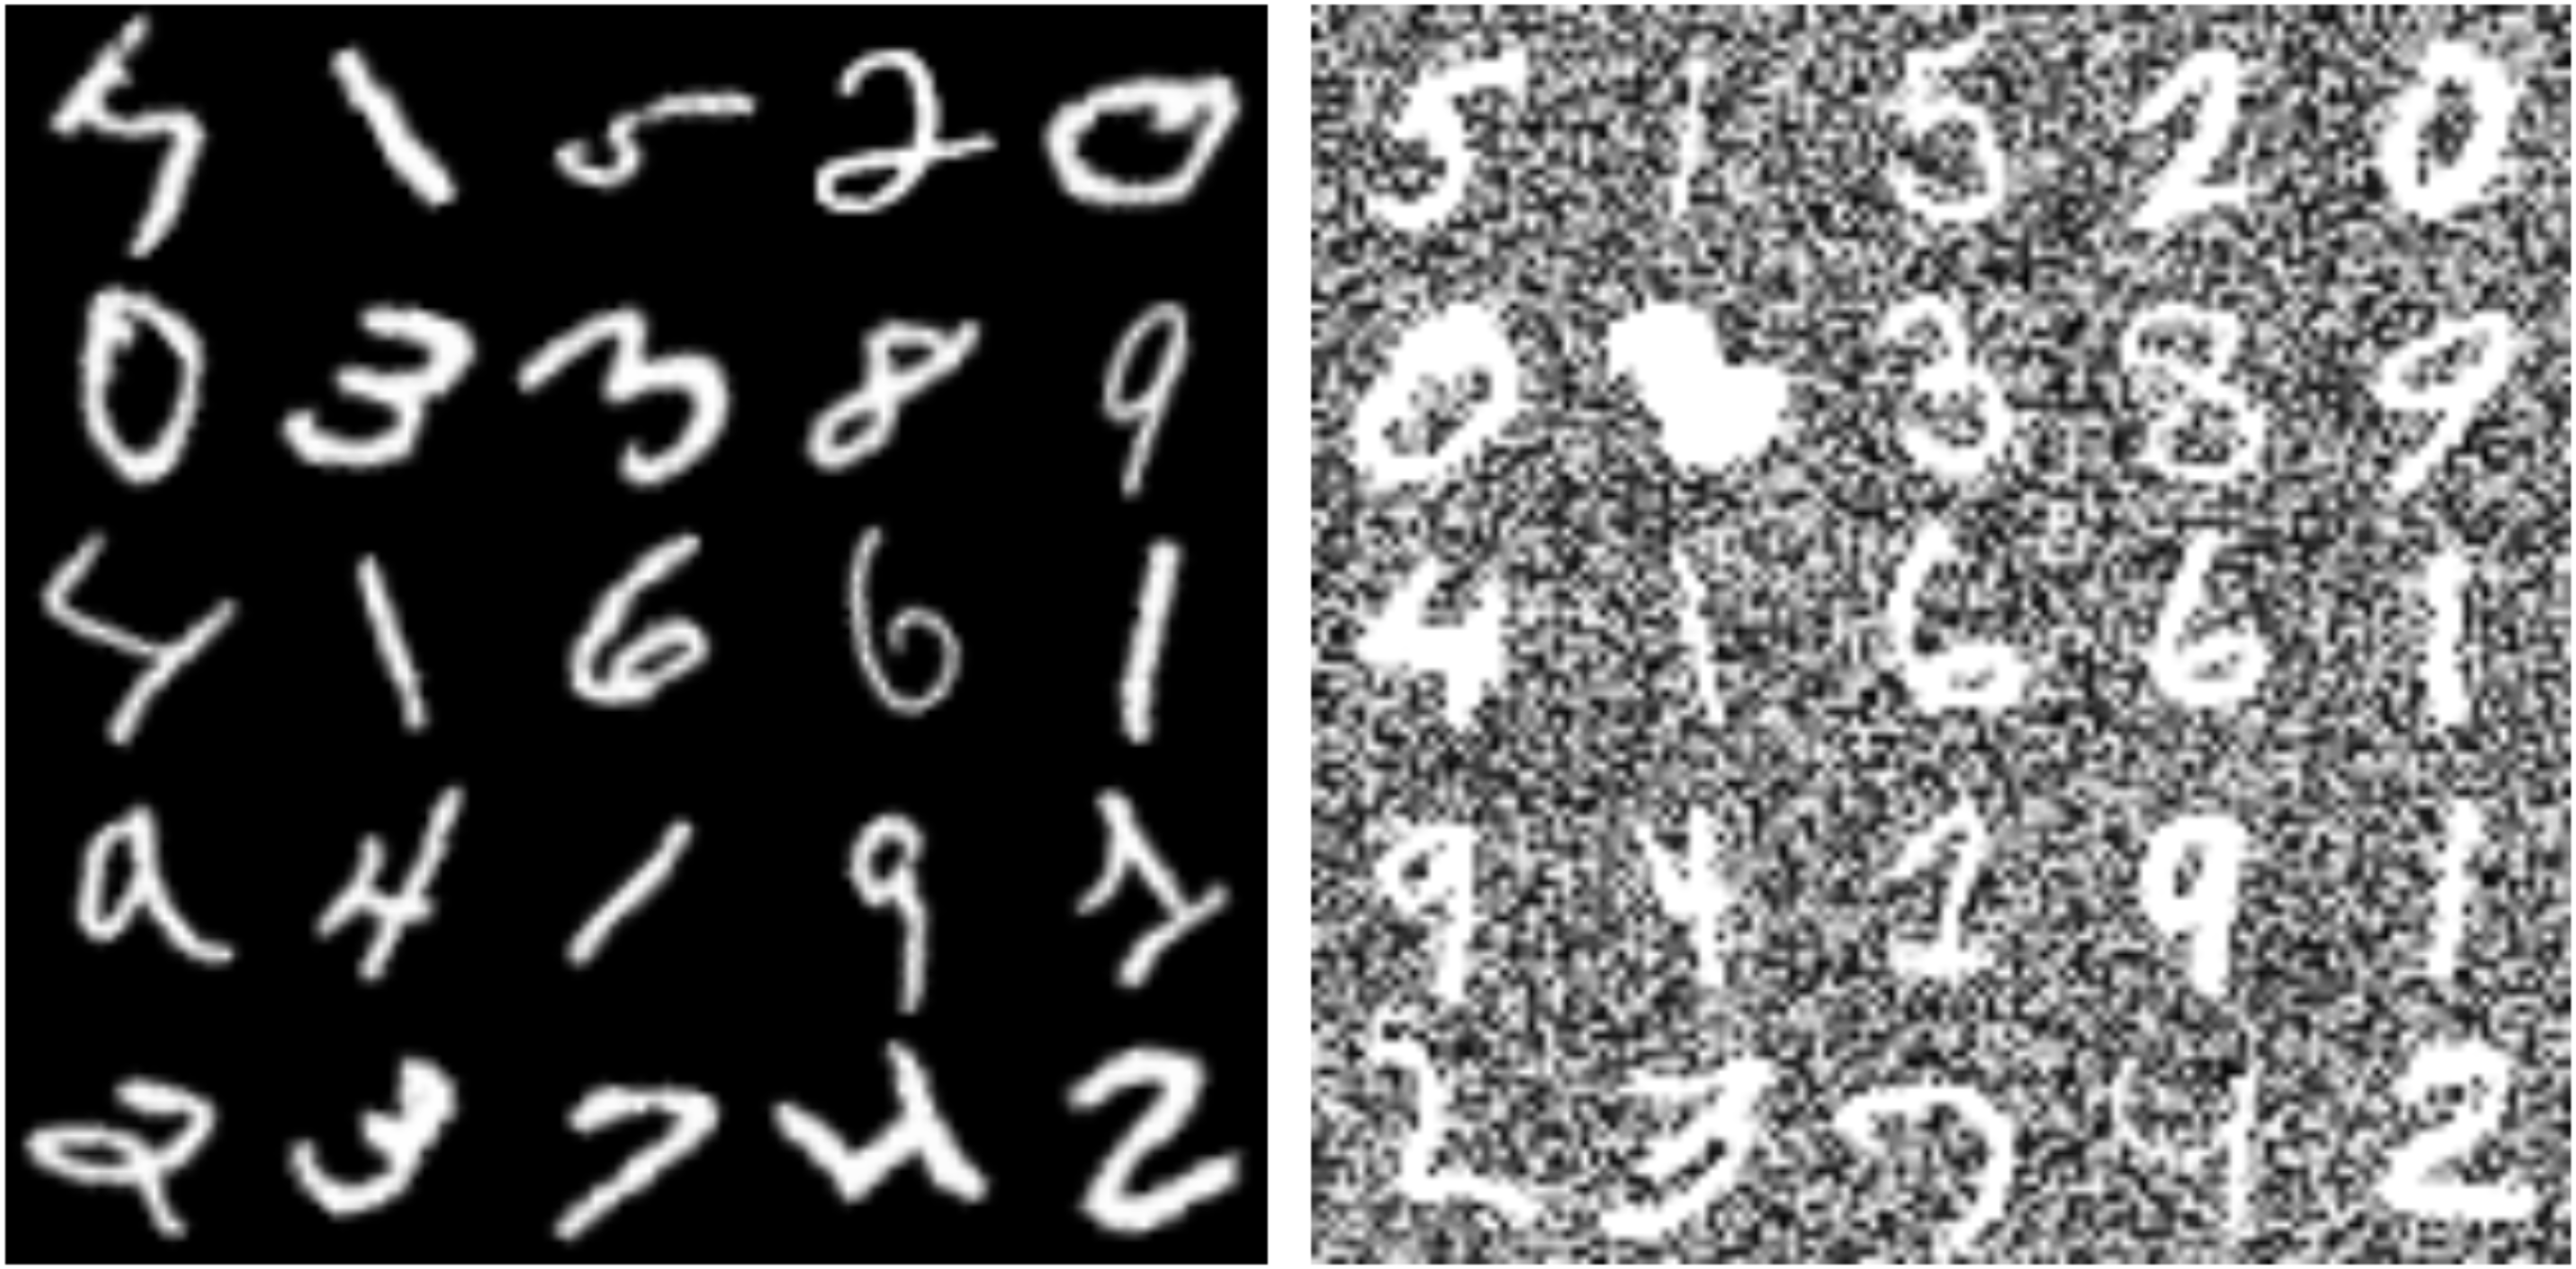
\includegraphics[width=\linewidth]{figures/noisy_mnist}
\caption{Зашумленные изображения из набора данных MNIST}
\label{fgr:1}
\end{figure}


\subsection{Анализ нелинейных зависимостей в задаче фильтрации шума}

Проведем сравнение качества Deep CCA и CCA на задаче классификации зашумленных цифровых изображений, представленных на рис.~\ref{fgr:1}. Для этого используется набор данных MNIST~\cite{MNIST}, который состоит из 70~000 цифровых изображений $28 \times 28$ образцов рукописного написания цифр. Предлагается получить два новых набора данных $\bX$ и $\bY$ следующим образом. Первый набор получается поворотом исходных изображений на угол в диапазоне $[\frac{-\pi}{4}, \frac{\pi}{4}]$. Для получения второго набора данных для каждой картинки из первого набора данных ставится в соответствие случайным образом картинка с той же цифрой, но с добавлением независимого случайного шума, распределенного равномерно на отрезке $[0,1]$.

\begin{table}[!bp]
\caption{Точность классификации линейного SVM для алгоритмов Deep CCA и CCA}
\centering
\begin{tabular}{l|cc}
\hline
	Скользящий контроль & Deep CCA ($L=3$) & CCA \\  \hline
	Валидация & 92,74\%  &  76,21\%\\
	Тест & 92,14\% & 76,07\% \\
	\hline
\end{tabular}
\label{tbl:1}
\end{table}

Применив к двум новым наборам данных DeepCCA или CCA, получаем новое низкоразмерное признаковое пространство, которое игнорирует шумы в исходных данных. Таким образом, получаем функции кодирования $\varphi_1$ и $\psi_1$ для исходных наборов данных. На новых признаках, полученных разными моделями (DeepCCA и CCA), для первого набора данных, то есть на данных после применения функции кодирования $\varphi_1$ к первому набору исходных данных, обучим линейный SVM-классификатор. Показателем эффективности будет точность классификации линейного SVM на тестовых данных. В случае построения адекватного скрытого пространства полученные образы объектов будут линейно разделимы. Результаты эксперимента приведены в табл.~\ref{tbl:1}. Модель Deep CCA представляет собой нейронную сеть с $L=3$ скрытыми слоями. Точность классификации нелинейной модели существенно выше линейного алгоритма CCA.

\subsection{Анализ нелинейных моделей для восстановления изображений}
Для анализа процедуры согласования проведен вычислительный эксперимент с предложенными нелинейными моделями.
Для снижения размерности пространства используются нейросетевые модели автокодировщика c согласованием скрытого пространства~\eqref{concordance}.
В качестве базовых моделей используются модель автокодировщика без согласования скрытых пространств, а также линейный PLS. В качестве исходного набора данных используется набор данных MNIST~\cite{MNIST}. Каждое изображение поделено на левую и правую части, как показано на рис.~\ref{fgr:3}. Модель по левому изображению восстанавливает правое изображение.

\begin{figure}[!tp]
\centering 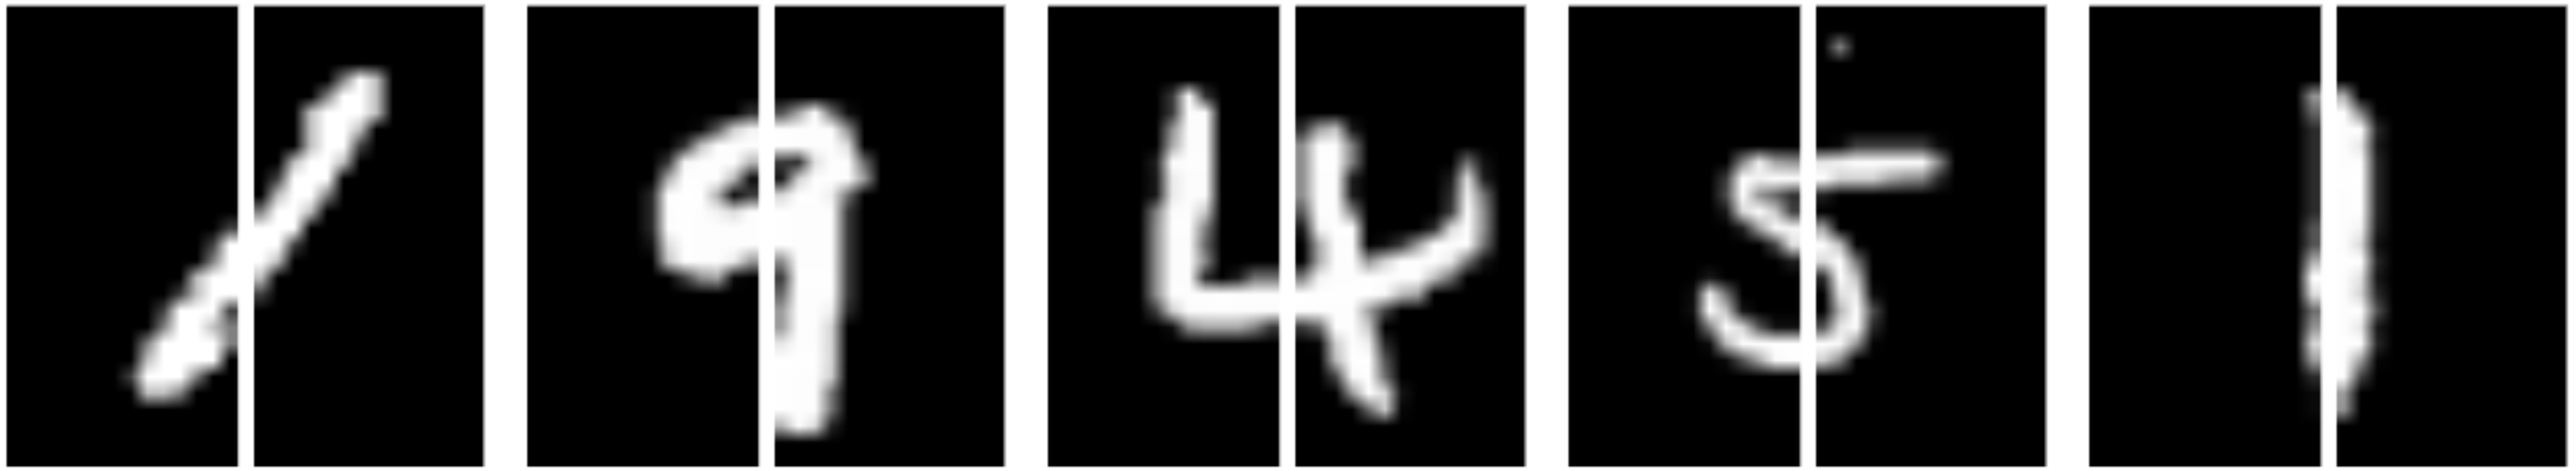
\includegraphics[width=\linewidth]{figures/left_right_mnist}
\caption{Набор данных MNIST, в котором каждое изображение разделено пополам}
\label{fgr:3}
\end{figure}

Модель EncNet1~--- нейронная сеть с нелинейными функциями активации, которая обучается на данных после преобразования их автоэнкодером. Модель LinNet1~--- нейронная сеть с одним линейным слоем, которая также обучается на преобразованных данных. Для EncNet1 и LinNet1 автоэнкодеры для объектов и ответов используют совместную функцию потерь, которая связывает выходы энкодеров. Модели EncNet2 и LinNet2 устроены аналогично EncNet1 и LinNet1 соответственно, но в автоэнкодерах нет совместной функции потерь. Модель DumbNet~---  нейронная сеть, которая обучается на исходных данных и имеет такую же структуру, что и EncNet, то есть имеет такое же число слоев и в каждом слое такое же количество нейронов, что и у EncNet.

\begin{table}[!bp]
\caption{Квадратичная ошибка для нелинейных моделей в задаче восстановления правой части изображения по левой}
\centering
\begin{tabular}{l|cccccc}
\hline
	& EncNet1 & LinNet1 & EncNet2 & LinNet2 & DumbNet & PLS\\  \hline
	Число параметров, тыс. & 283 & 239 & 283 & 239  & 283 & --\\ 
	Ошибка на тесте & 0,147 & 0,235 & 0,149 & 0,236 & 0,128 & 0,188 \\ 
	\hline
\end{tabular}
\label{tbl:2}
\end{table}

Для оценки качества моделей вычислялась среднеквадратичная ошибка. Примеры восстановленных изображений показаны на рис.~\ref{fgr:2}. Качество моделей, а также их сложность представлены в табл.~\ref{tbl:2}. 
На рис.~\ref{fgr:2} продемонстрировано, что предложенные модели EncNet и LinNet позволяют получить более четкие и различимые изображения, в отличие от базовой нелинейной модели DumbNet и линейной модели PLS.
Несмотря на заметное улучшение визуального качества изображений, ошибка предложенных моделей выше, чем у модели DumbNet. 
Авторы предполагают, что это связано с тем, что среднеквадратичная ошибка оказалась неадекватной метрикой в пространстве изображений.
Нахождение оптимальной метрики для оценки качества предложенных алгоритмов может быть одним из возможных направлений развития текущей работы.

\begin{figure}[!tp]
\centering 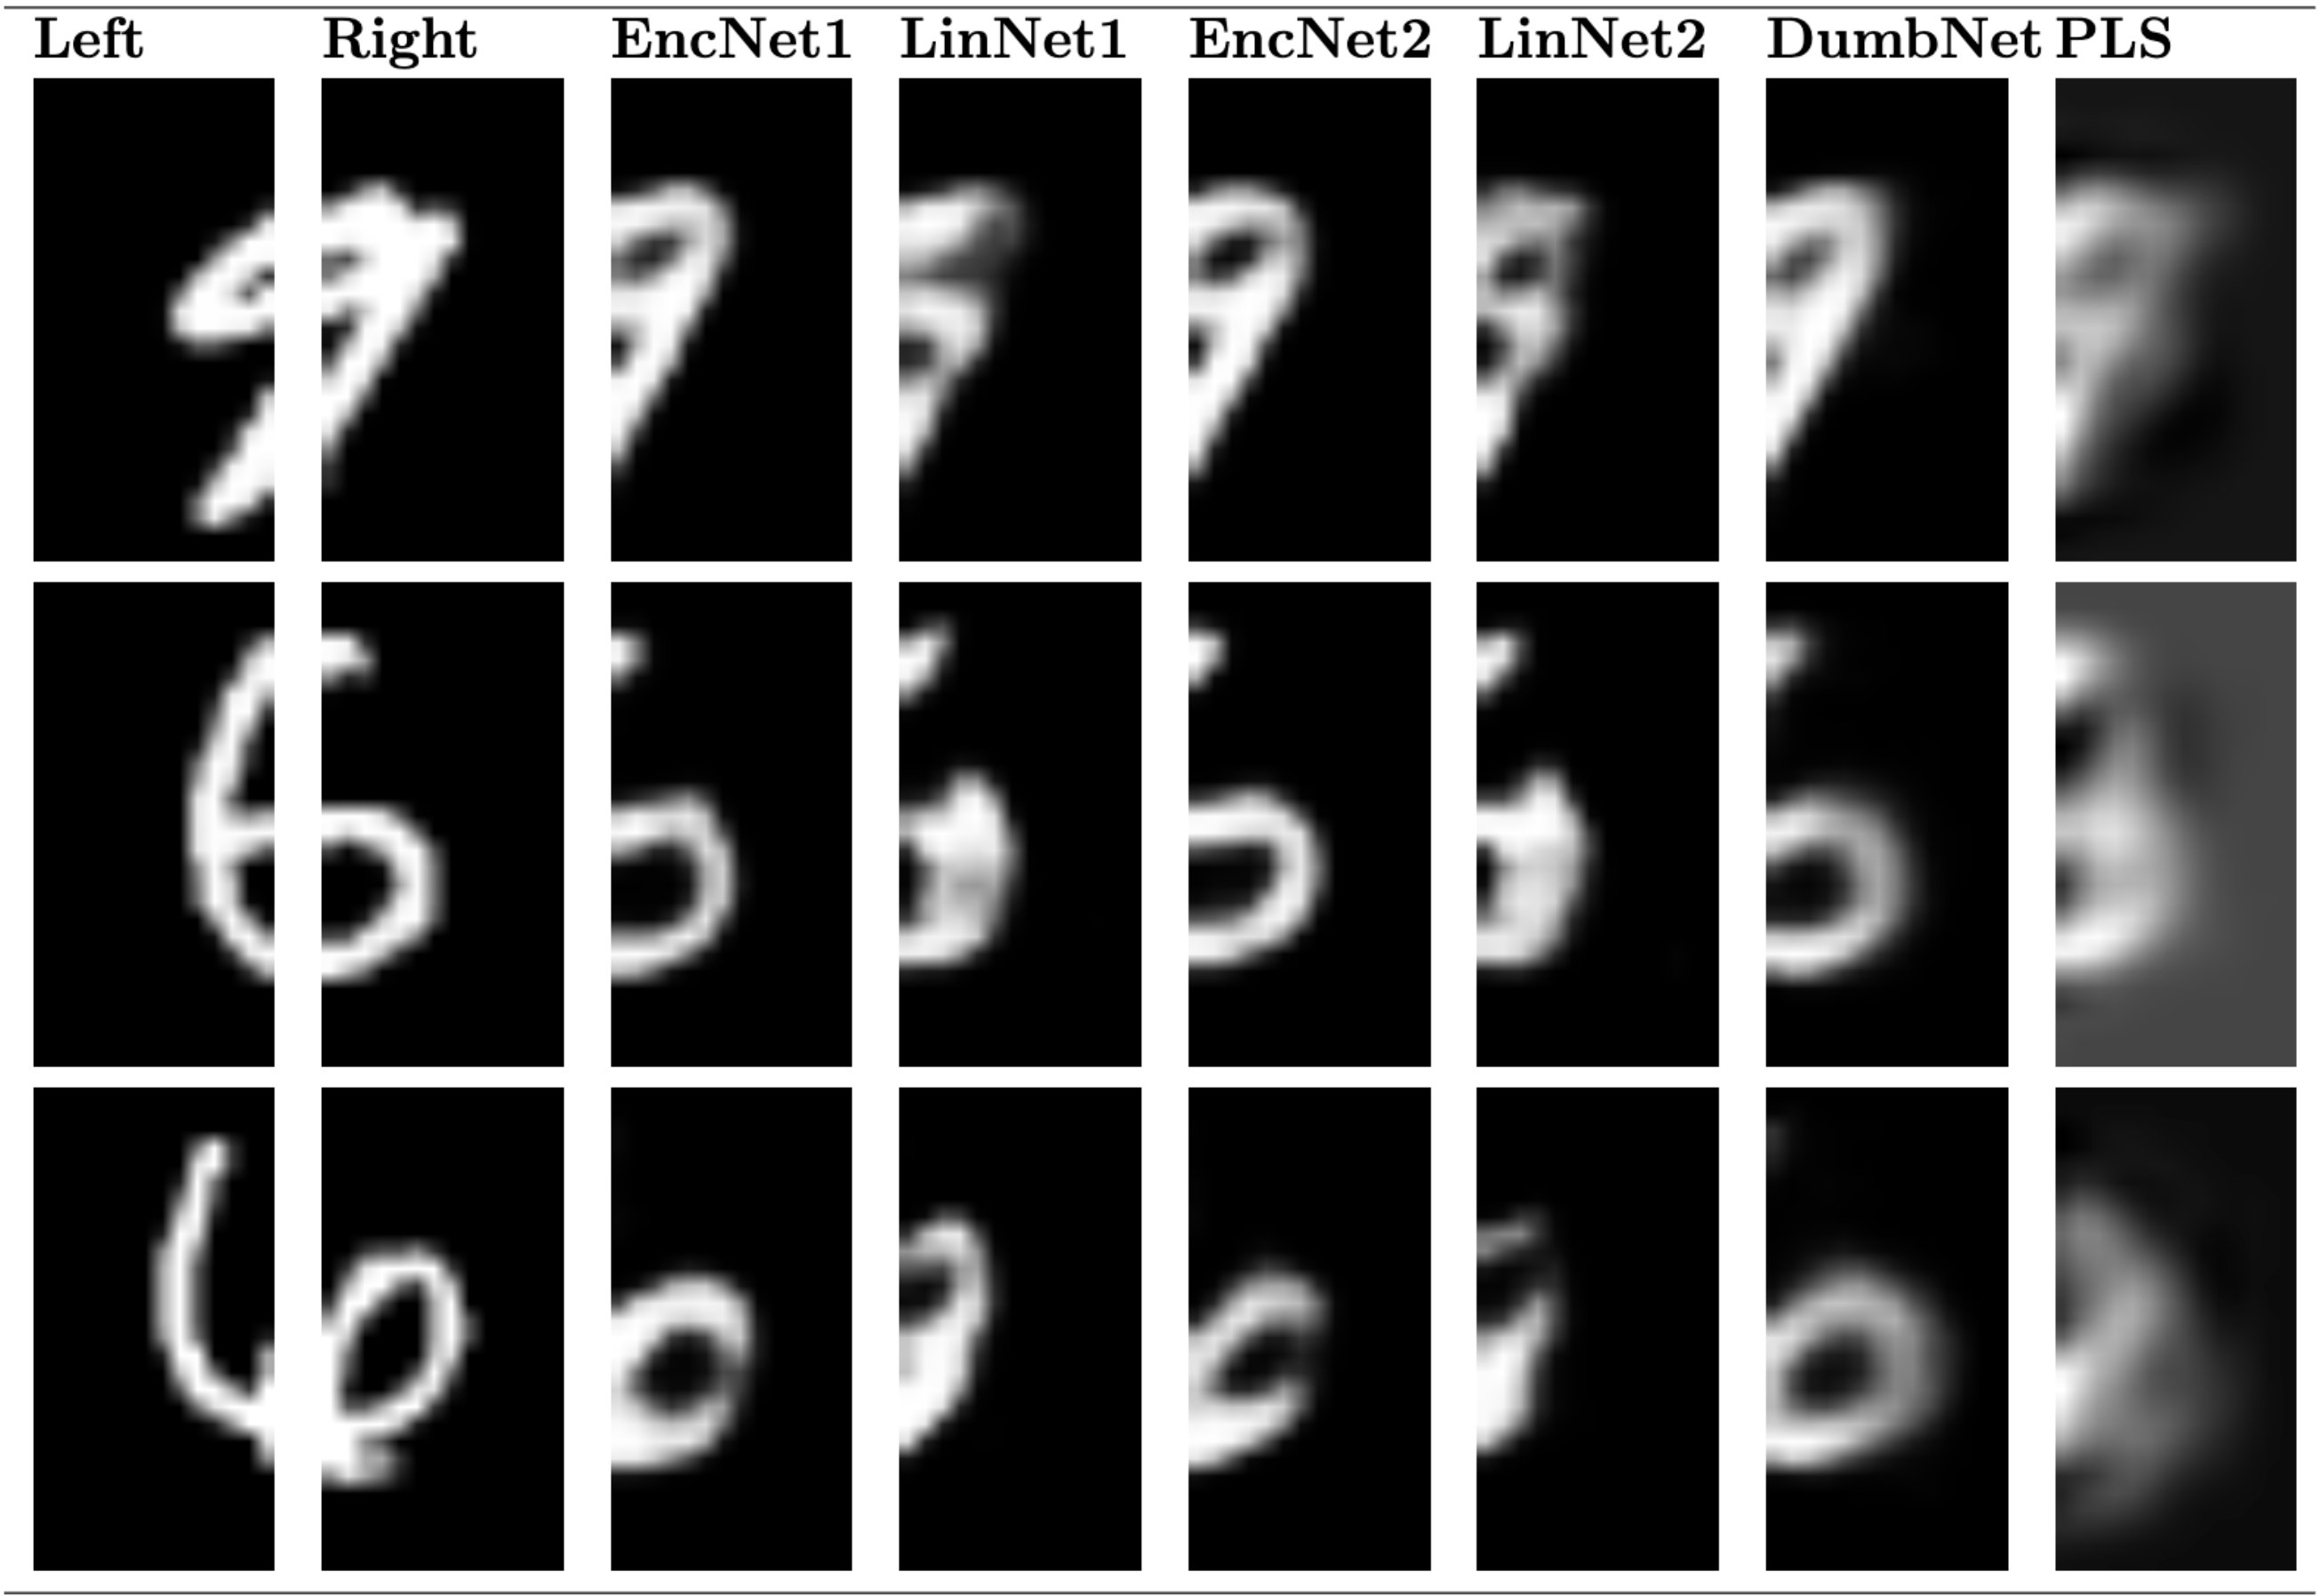
\includegraphics[width=\linewidth]{figures/mnist_preds}
\caption{Пример реконструкции правой части изображения по левой для рассматриваемых моделей}
\label{fgr:2}
\end{figure}

\section{Заключение}
В работе рассмотрена задача восстановления для сложноорганизованной целевой переменной.
Рассмотрены линейные модели согласования образов объектов в скрытом пространстве.
При наличии сложных нелинейных зависимостей между независимой и целевой переменной сложности линейной модели оказывается недостаточно.
Для построения точного прогноза приводятся нелинейные обобщения рассматриваемых линейных методов.
В экспериментах на реальных данных изображений рукописных цифр показана адекватность рассматриваемых нелинейных моделей, а также проведен анализ различных способов согласования.

\bibliographystyle{unsrt}
\begin{thebibliography}{99}

\bibitem{overview_pls}
\textit{Rosipal R., Kramer N., Graves A.} Overview and recent advances in partial least squares~// Subspace, Latent Structure and Feature Selection: International Statistical and Optimization Perspectives Workshop. -- Springer, 2005. P. 34--51.

\bibitem{overview_nonlinear_pls}
\textit{Rosipal R.} Nonlinear partial least squares: An overview~// Chemoinformatics and Advanced Machine Learning Perspectives. -- IGI Global, 2011. P. 169--189.

\bibitem{1figures}
\textit{Nguyen D. V., Rocke D. M.} Tumor classification by partial least squares using microarray gene expression data~// Bioinformatics, 2012.  Vol.~18. P.~39--50. 

\bibitem{btc519}
\textit{Worsley K. J.} An overview and some new developments in the statistical analysis of pet and fmri data~// Human Brain Mapping, 1997. Vol.~5. P.~254--258.

\bibitem{PLS_in_strategic_management}
\textit{Hulland J. S.} Use of partial least squares (pls) in strategic management research: A review of four recent studies~// Strategic Management Journal, 1999. Vol.~20. P.~195--204.

\bibitem{PLS_application}
\textit{Shalamu Abudu P. E., Pagano T. C.} Application of partial least-squares regression in seasonalstreamflow forecasting~// Journal of Hydrologic Engineering, 2010. Vol.~15. P.~612--623.

\bibitem{cca_alg}
\textit{Szedmak S. R., Hardoon D. R., Shawe-taylor J. R.} Canonical correlation analysis: An overview with application to learning methods~// Neural computation, 2004. Vol.~16. P.~2639--2664.

\bibitem{cca_apl1}
\textit{Schechner Y. Y., Kidron E., Elad M.} Pixels that sound~// IEEE Computer Society, 2005. Vol.~1. P.~88--95.

\bibitem{cca_apl2}
\textit{Sun S., Ji L., Ye J.} A least squares formulation for canonical correlation analysis~// Proceedings of the 25th international conference on Machine learning. -- ACM, 2008. P.~1024--1031.

\bibitem{PLS_nn}
\textit{Qin S. J., McAvoy T. J.} Nonlinear pls modeling using neural networks~// Computers Chemical Engineering, 1992. Vol.~16. P.~379--391.

\bibitem{PLS_rbf}
\textit{Chen D. Z., Yan X. F., Hu S. X.} Chaos-genetic algorithms for optimizing the operating conditions based on rbf-pls model~// Computers and Chemical Engineering, 2003. Vol.~27. P.~1393--1404.

\bibitem{PLS_ga}
\textit{Hiden M., McKay B., Montague G.} Non-linear partial least squares using genetic programming~// Genetic Programming. -- Morgan Kaufmann San Francisco, 1998. P.~128--133.

\bibitem{deep_cca}
\textit{Chen D. Z., Yan X. F., Hu S. X.} Deep canonical correlation analysis~// Proceedings of the 30th International Conference on Machine Learning. -- PMLR, 2013. P.~1247--1255.

\bibitem{kernel_cca}
\textit{Lai P. L., Fyfe C.} Kernel and nonlinear canonical correlation analysis~// International Journal of Neural Systems, 2000. Vol.~10. P.~365--377.

\bibitem{kernel_cca_appl}
\textit{Yan F., Mikolajczyk K.} Deep correlation for matching images and text~// Computer Vision and Pattern Recognition, 2015. Vol.~4. P.~3441--3450.

\bibitem{MNIST}
\textit{LeCun Y.,  Cortes C., Burges C.} The MNIST dataset of handwritten digits, 1998. \url{http://yann.lecun.com/exdb/mnist/index.html}.

\bibitem{source_code}
\textit{Yaushev F. Yu,  Isachenko R. V.} Модели согласования скрытого пространства в задаче прогнозирования. 2020. \url{https://github.com/Fyaushev/2020-Project-72}.
\end{thebibliography}

\end{document}

